\begin{refsection}
\chapter{Trees and Forests}

\begin{summary}
Trees introduce learning via recursive partitioning of the input variable space. Depending on the learning task, the algorithm used is either a classification tree or a regression tree, respectively. The inference of trees is fast but leads to models that are not stable and have high variance. To reduce the variance and increase stability, the upgrade of the tree-learning approach may construct a set of trees. We define two such procedures; one called bootstrap aggregation (bagging) and the other random forest.
\end{summary}

\section{Classification and Regression Trees (CART)}

Classification and regression trees, somehow surprisingly, conceptually relate to other advanced machine learning approaches, such as kernel methods, generalized linear models, and adaptive basis function models. While we have yet to discuss them, let us visit them briefly for some motivation. The (generalized) linear modelling paradigm, as introduced in the next lecture, assumes that the data generating process can be interpreted with a family of distributions whose parameters are in a (transformed) linear relationship with the input variables. These are parametric models. For kernel methods, the prediction takes the form of a weighted sum $f(\vect{x})=\vect{w}^\tr\vect{\phi}(\vect{x})$, where $\vect{w}$ is a weight vector and $\phi$ is a vector of similarities with an input example $\vect{x}$, such that
$$ \vect{\phi}(\vect{x}) = [\kappa(\vect{x},\vect{\mu}_1), \ldots, \kappa(\vect{x},\vect{\mu}_n)] $$
where $\vect{\mu}_k$ are either all the training data or some sample, and $\kappa$ is a kernel function. Kernel functions are, in general, defined in advance, and coming up with a good kernel is hard and may depend on the problem domain.

Learning kernel functions is on option, but is computationally expensive and requires a lot of data. An alternative approach is to forget about kernels, and instead infer useful features $\vect{\phi}(\vect{x})$ directly from the training data. This is an approach used by adaptive basis function model, which takes the form
$$ f(\vect{x})=w_0+\sum_{m=1}^{M} w_m\phi_m(\vect{x}) $$
where $\phi_m(\vect{x})$ is the $m$-th basis function inferred from the training data. The basis functions are parametric, so that we can write $\phi_m(\vect{x})=\phi_m(\vect{x};\vect{v}_m)$, where $\vect{v}_m$ are the parameters of the basis function itself. The CART approach can be viewed as a special case of adaptive basis function model. CART recursively partitions the input space and defines a simplified local model in each resulting region. Recursive partitioning can be represented as a tree, where partitioning conditions are stored in internal nodes and region models in the leaves. The model takes the following form
\begin{align}
f(\vect{x}) & = \mathbb{E}[y|\vect{x}] \\
 & = \sum_{m=1}^M w_m \mathbb{I}(\vect{x}\in R_m) \\
 & = \sum_{m=1}^M w_m\phi(\vect{x};\vect{v}_m)
\end{align}
where $R_m$ denotes the $m$'th region and $w_m$ is, simplified, the main response in the region. The set $\vect{v}_m$ encodes the choice of the variable to split on and the related threshold value in the path from the root of the tree to the specific leaf. Notice that in CART the regions do not overlap, and that the training example falls in only and exactly one of the constructed regions. The region splits are defined on exactly one of the variables and are thus axis parallel.

\subsection*{Basic Idea}

From the viewpoint of model construction and compared to generalized linear models, kernel methods, and inference of adaptive basis function models, CART introduces a fundamentally different modelling paradigm. One that assumes that the data generating process can be interpreted as a partition of the input variable space into homogeneous (pure) regions -- regions where there is little or no uncertainty left about the target variable. For regression, the target variable for the data instances within this region is almost constant (see Fig.~\ref{fig:trees-sin}). For classification, a majority of data instances in the region have the same value of the target variable.

\begin{figure}
\centering{
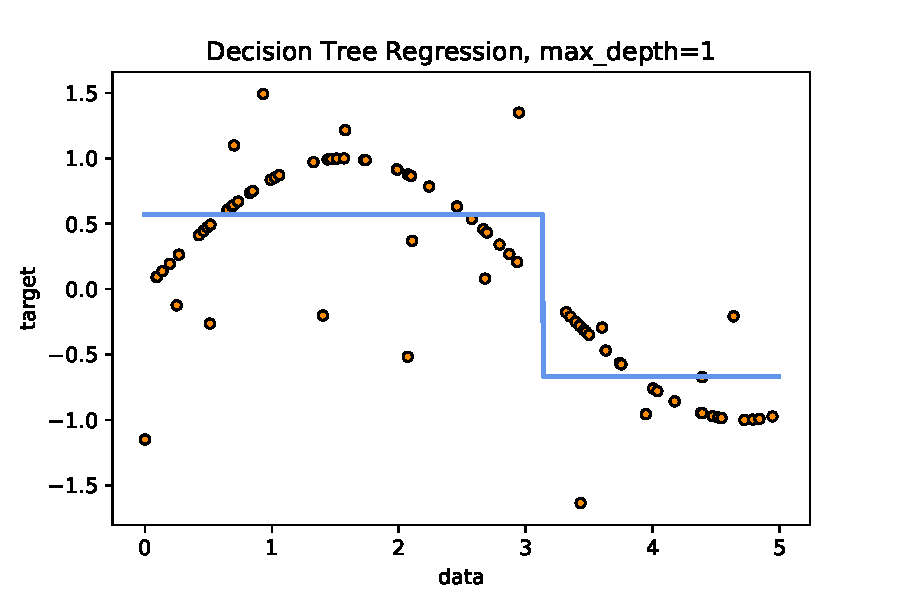
\includegraphics[width=0.47\linewidth]{figures/trees-sin-1.pdf}
\hfill
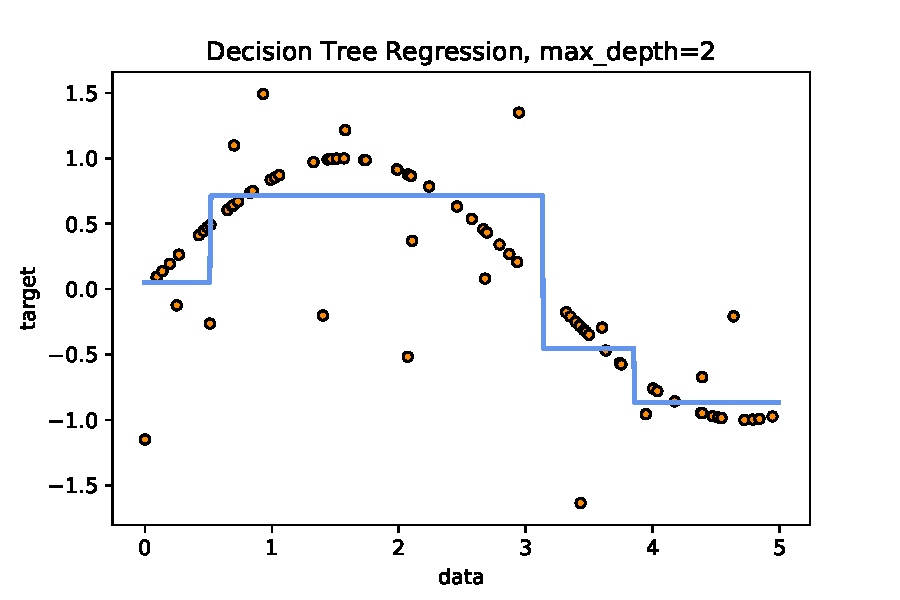
\includegraphics[width=0.47\linewidth]{figures/trees-sin-2.pdf}

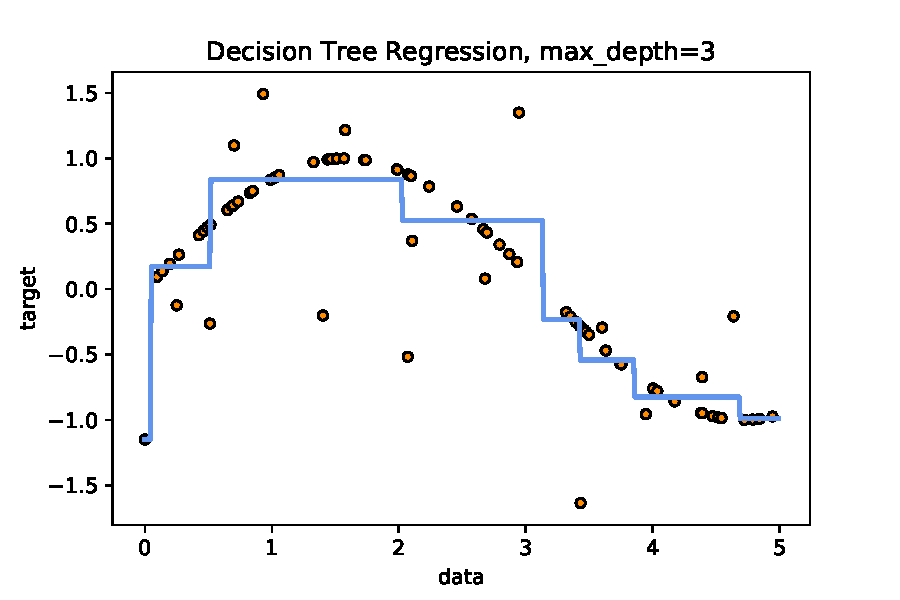
\includegraphics[width=0.47\linewidth]{figures/trees-sin-3.pdf}
\hfill
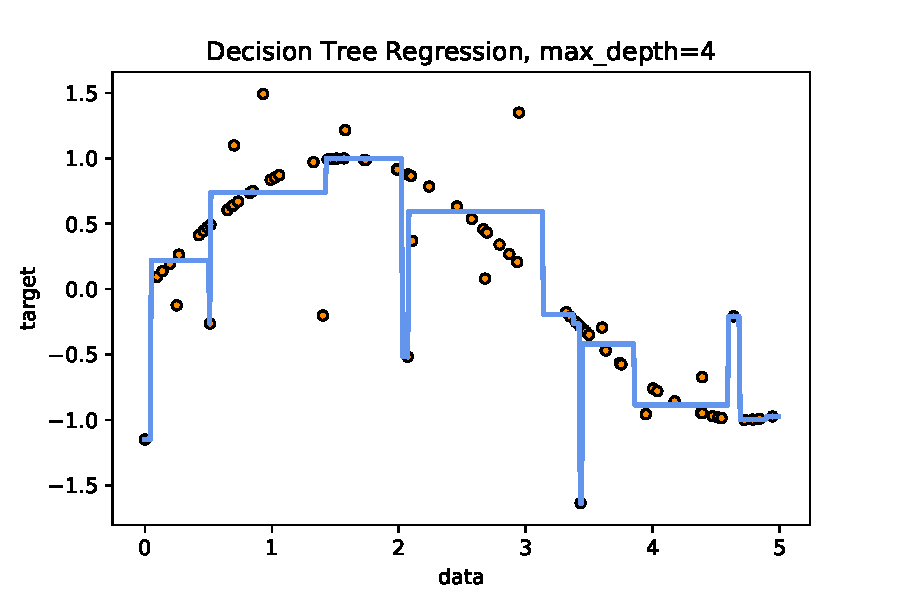
\includegraphics[width=0.47\linewidth]{figures/trees-sin-4.pdf}
}
\caption{Regression trees fitted on data generated by a sine function with some noise. While the tree adapts well to the training data, its ability to overfit the training data is visible already with trees with of maximum depth of 4 (lower right).}
\label{fig:trees-sin}
\end{figure}

\begin{figure}[htbp]
\centering{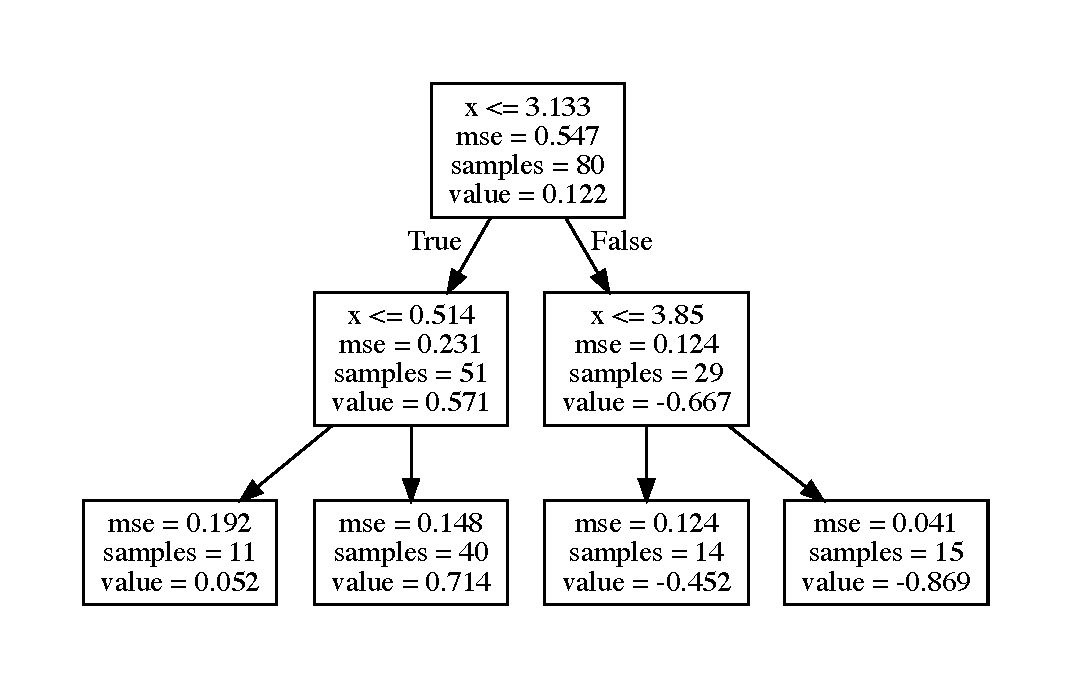
\includegraphics[width=0.7\linewidth]{figures/trees-rtree}}
\caption{A regression tree with maximum depth of 2 from the data from Fig.~\ref{fig:trees-sin}.}
\label{fig:fig:trees-sin-2}
\end{figure}

\subsection*{The CART Algorithm}

Finding the optimal partitioning of the input variable space is in general NP-complete, even if using axis-parallel splits only. That is, it is infeasible to check all possible partitions. Instead, we will consider a greedy algorithm (CART) that is based on binary recursive partitioning of the input space, at each step choosing the best possible split (according to some pre-selected criterion). Notice that this algorithm does not use any look-ahead, and while such algorithms were studied in the literature, they are not used in practice. A simplified and abstracted CART algorithm is encoded as Algorithm~\ref{alg:cart}.

\begin{algorithm}
\begin{algorithmic}[1]
\Procedure{fitTree}{$\DS$}
\State $(\DS_L, \DS_R, criterion) \gets split(\DS)$
\State $node \gets createNode(criterion, \DS)$
\If {stoppingCriterionMet(criterion, $\DS$)} \Return node \EndIf
\State $node.L \gets fitTree(\DS_L)$
\State $node.R \gets fitTree(\DS_R)$
\State \Return node
\EndProcedure
\end{algorithmic}
\caption{CART}\label{alg:cart}
\end{algorithm}

The CART algorithm uses several functions that require explanation:
\begin{itemize}
\item {\em createNode()}: This function creates an object that represents a tree node, which essentially stores the criterion on which the data in the node is split, and a possible reference to the data instances that are pertinent to the node. If a suitable node split is found, the node stores the information on its to siblings. Note that, as introduced above, the CART algorithm would construct binary trees.
\item {\em split()}: The assumption here is that features are numerical or at least ordinal. We order every feature based on possible splits (based on unique values in the data, so we have a finite number of possible splits). And then we basically go through all possible feature-split combinations to find the one that is optimal according to our splitting criterion -- the one that minimizes the sum of the cost of the left and right subtrees. Possible splitting criteria are discussed below.

\item {\em stoppingCriterionMet()}: The stopping condition, also referred to as {\em pre-prunning} of the trees, can be one or more of the following:
\begin{itemize}
\item The partition is sufficiently homogeneous/pure. In particular, there is no point in splitting further if we have perfect homogeneity (all observations have the same value).
\item The gain $\Delta$ of splitting the data set in the current node (relative to stopping criterion) is below some pre-determined threshold, where
$$ \Delta = \cost(\DS) = \cost(\DS)-\left({|\DS_L|\over |\DS|}\cost(\DS_L) + {|\DS_R|\over |\DS|}\cost(\DS_R)\right)$$
\item The algorithm has reached pre-determined maximum tree depth.
\item Splitting the data set in the node would yield a leaf with number of observations below some pre-determined minimum.
\end{itemize}
\end{itemize}


\subsection*{Choice of the Splitting Criterion}

At each internal node, the inference methods for the trees splits the training data set $\DS$ pertinent to the node to maximize some splitting criterion. The split is performed using a single feature from the training data set and forming a condition on the value of this feature that evaluates to true or false. According to this condition, the data $\DS$ is then split to two data sets, each pertinent to one of the two siblings of the node. This type of splitting results in a binary tree. Notice that other, non-binary, splitting mechanisms could be used, but they would lead to over-fragmentation of the data, increase the variance, and lead to increased overfitting.

Splitting criteria are related to data set purity, costs, loss, or estimated errors, and have to specifically address the type of the target feature, this being either numerical or discrete. Note that since the introduction of classification and regression trees, many different criteria were proposed and while, at least on the surface, these take different forms, the practical differences regarding overall accuracies and ordering of the features are often neglectable. The costs of the splitting is most often estimated for each of the resulting siblings (leaves), and then weighted according to the estimated probability that the data instance will fall in one of the two constructed regions
$$ \cost(node, criterion) = {|\DS_L|\over |\DS|}\cost(\DS_L) + {|\DS_R|\over |\DS|}\cost(\DS_R) $$

For regression trees, the most often used splitting criterion is the mean squared error of predicting with the subtree mean
$$ cost(\DS) = \sum_{i\in\DS}(y_i-\overline{y})^2 $$
where $\overline{y} = {1\over|\DS|}\sum_{i\in\DS}y_i$ is the mean of the target variable in the resulting data set.

Many more splitting criteria were proposed for the classification setting, and most of them rely on estimating class-conditional probabilities
$$ \hat{\pi}_c = {1\over|\DS|}\sum_{i\in\DS}\mathbb{I}(y_i\equiv c) $$
For instance, we can measure the {\em entropy} (or {\em deviance}) of the resulting data set
$$ \mathbb{H}(\hat{\vect{\pi}}) = -\sum_{c=1}^C \hat{\pi}_c \log \hat{\pi}_c $$
or can measure the expected error rate in the form of a {\em gini index}
$$ \sum_{c=1}^C \hat{\pi}_c (1-\hat{\pi}_c) = \sum_c \hat{\pi}_c - \sum_c \hat{\pi}_c^2 = 1 - \sum_c \hat{\pi}_c^2 $$
where $\hat{\pi}_c$ is the probabilty a random entry in the leaf belongs to class $c$, and $1-\hat{\pi}_c$ is the probability for this entry to be misclassified. Other criterion may include information gain, information gain ratio, chi-squared test, and similar. Note that with all the above criteria, splitting the training data set will never decrease the quality (and increase the cost) and in the worst case the quality will remain the same if the node's data set is already homogeneous. Notice that we are estimating all the costs on the training set and thus potentially overfitting the data.

\subsection*{Discussion}

There are several issues with growing and using the classification and regression trees. The trees have some advantages and many disadvantages. While, on their own, the trees are rather mediocre predictors, their enhancements in terms of ensembling discussed in the following sections of this chapter elevate them to at least a formidable baseline, if not state-of-the-art approach. Therefore, let us first review some of the issues that are pertinent to development and utility of CART, that is, induction of single trees.

\begin{description}
\item[Interpretation.] Decision trees are easy to interpret. In fact, according to the current research, the interpretability of trees is only behind decision tables and individual rules when it comes to non-expert users. This is somewhat marred by the fact that the standard decision tree algorithms are susceptible to changes in the inputs. A small change in the training data set can result in a substantially different tree. What good is an in-depth interpretation of the model if this is inherently unstable? We can mitigate instability by using bootstrapping to check if the algorithm produces stable trees before proceeding with the analysis. Also, learning a (stable) tree that mimics a more complex model such as a tree ensemble and neural networks is one of the most common approaches to explaining how the complex model works. This approach, though, has gained recent criticism that if one is after the explanation, one should primarily build interpretable models in the first place, and not represent complex models with simple ones~\citep{Rudin2019}.

\item[Low computational complexity.] Trees are fast to training and very fast in prediction. They scale well to large data sets. The only exception to this observation is in treatment of sparse data, that is, data with many unknown values. A thorough treatment of unknown values may invalidate the divide-and-conquer approach with the passing of full data sets to leaves and potentially visiting the entire tree when predicting. A potential remedy of this side effect is to impute the missing values before training or prediction.

\item[Weak inductive bias.] Compared to more sophisticated methods, including ensembles of trees and neural networks, classification and regression trees have a relatively weak inductive bias. That is, they will not perform the best (or close to) in terms of predictive quality on most practical problems. The two main issues are a {\em lack of smoothness} and {\em difficulty of capturing additive relationships}. See~\citep{ESL} for further details.

\item[Possible complex treatment of categorical input variables.] When splitting a predictor having $q$ possible unordered values, there are $2^{q-1}-1$ possible partitions of the $q$ values into two groups and the computations become prohibitive for large $q$. For example, consider the treatment of postal codes in the data sets. There are possible heuristic approaches to cope with such cases, though. For binary target variables, we can order the predictor classes according to the proportion falling in outcome class 1. Then we split this predictor as if it were an ordered predictor. One can show this gives the optimal split, in terms of cross-entropy or Gini index, among all possible splits. This result also holds for a quantitative outcome and squared error loss—the categories are ordered by increasing the mean of the outcome. The proof for binary outcomes is given in Breiman et al.~\citep{Brieman1984} and Ripley~\citep{Ripley1996}; the proof for quantitative outcomes can be found in Fisher~\citep{Fisher1958}. For multicategory outcomes, no such simplifications are possible, although various approximations have been proposed~\citep{Loh1988}.

The partitioning algorithm tends to favor categorical features with many values; the number of partitions grows exponentially in $q$, and the more choices we have, the more likely we can find an (arbitrarily) good one for the data at hand. This can lead to severe overfitting if $q$ is significant, and such variables should either be avoided or some preprocessing by means of a grouping of similar feature values, such as clustering, should be used. Also, note that dummy (one-hot) encoding of categorical variables can lead to the opposite problem of individual binary variables not being selected over many features represented encoded variables.

\item[The benefits of binary splits.] Rather than splitting each node into just two groups at each stage, we might consider multiway splits into more than two groups. While this can sometimes be useful, it is not a good general strategy. The problem is that multiway splits fragment the data too quickly, leaving insufficient data at the next level down. Hence we would want to use such splits only when needed. Since multiway splits can be achieved by a series of binary splits, the latter is preferred.

\item[Treatment of missing values.] Suppose our data has some missing predictor values in some or all of the variables. We might discard any observation with some missing values, but this could lead to severe depletion of the training set. Alternatively, we might try to fill in (impute) the missing values, with say the mean of that predictor over the non-missing observations. For tree-based models, there are two better approaches. The first is applicable to categorical predictors: we make a new category for “missing.” From this, we might discover that observations with missing values for some measurement behave differently than those with non-missing values. The second more general approach is the construction of surrogate variables. When considering a predictor for a split, we use only the observations for which that predictor is not missing. Having chosen the best (primary) predictor and split point, we formed a list of surrogate predictors and split points. The first surrogate is the predictor and corresponding split point that best mimics the split of the training data achieved by the primary split. The second surrogate is the predictor and relevant split point that does second best, and so on. When sending observations down the tree either in the training phase or during prediction, we use the surrogate splits in order, if the primary splitting predictor is missing. Surrogate splits exploit correlations between predictors to try and alleviate the effect of missing data. The higher the correlation between the missing predictor and the other predictors, the smaller the loss of information due to the missing value.

\item[Tree pruning.] If the tree is allowed to grow until the leaves are entirely (or nearly) homogenous, we are likely to be overfitting. In some cases that is desirable - we will see such an example later with random forests, where we want an individual tree in the ensemble to include little modelling bias. However, in most cases, it is not. To prevent overfitting, we can carefully tune the stopping criteria. However, growing the entire tree and then post-processing it by {\em pruning} individual branches can sometimes lead to better results. The basic idea is to go over each split and check if not making that split would not result in a significant increase in error.
Additionally, we can use cross-validation to prune based on an estimate of the generalization error, making the process more robust. Note that cross-validation could (should), in theory, also be used when growing the tree. The reason why we make splits based on what is essentially training set error is that cross-validation would be computationally infeasible in most practical scenarios.

\item[Model trees.] As an alternative to reporting on average values in tree leaves, we can use non-trivial models. Many approaches combine trees with generalized linear (additive) models in the leaves. This can lead to improved results in problems that are a combination of crisp rules and (local) linear behavior while retaining most of the interpretability. However, it comes at the cost of computational complexity because it requires a more complex model evaluation when splitting the tree.

\item[Oblique feature space splitting.] Axis-parallel partitioning**: Most tree-based algorithms (including the one described above) limit themselves to axis-parallel splits. This can lead to very complicated trees if the boundaries between homogeneous regions do not follow this assumption. As an alternative, non-axis-parallel (oblique) algorithms have been developed. However, this comes at the cost of interpretability and computational complexity.
\end{description}

\section{Bagging}

Before we proceed with random forests, we will first introduce a component of random forests that has more general applicability. {\em Bagging} (Bootstrap Aggregation) is a technique that can improve the predictive quality of any models, in particular when the data set is small and/or we are dealing with a high-variance model that can easily overfit the training data. A prime example of such a model is a non-pruned tree.

The basic idea is straightforward: instead of using our model $\hat{f}$ that was trained on all the training data, we take $B$ bootstrap samples of the training data and re-train the model on each sample, resulting in $B$ models $\hat{f}_b$. The bootstrapped prediction is the aggregate (average) of the individual bootstrap models:

$$\hat{f}_{\text{boot}}(\vect{x}) = \sum_{b=1}^B {1\over B} \hat{f}_b(\vect{x}).$$

In essence, we are using the bootstrap, where the functional of the data is the model's prediction for $\vect{x}$. And, as we already know, the sampling error can be made arbitrarily small by increasing $B$.
%TODO: this last sentence not clear, why would we already know this?
%TODO: what is a functional?

\subsection*{Why Does Bagging Work?}

Note that most of the arguments we state here are from \citep{Grandvalet2004}. Some authors, including \citep{ESL}, claim that the bagging estimate will be the same as the original model if the model is linear. That does not imply that bagging will produce the same estimate if used on linear regression. Overall, there is little rigorous theoretical justification of why bagging should work, but there is ample empirical evidence that it often does work. Here we will offer some empirical justification for the underlying mechanisms that make bagging work (and sometimes fail).

Grandvalet (2004) argues that bagging equalizes the influence of individual points on the prediction. As the most influential points (points with high leverage) are typically outliers and have a bad influence on predictive quality, reducing their influence will improve performance by reducing the variance. This is a more general explanation to the more common explanation that bagging improves predictions because it reduces variance, in particular, because bagging can also increase variance. That is, if points of high leverage have a positive influence, bagging will decrease predictive quality.

One implication of the above is that models, where all points have the same or similar leverage, would not benefit from bagging. Similarly, models, where a single point has very little effect on the prediction, would also not benefit from bagging (robust models such as regularized regression or models that already contain some sort of bagging, such as random forests, which we discuss below). Therefore, high-variance models, such as non-pruned trees, is where we would expect the most benefit.

A prototypical example where all points have the same leverage (and bagging does nothing) is predicting with the training set average. With enough bootstrap samples, every point will be included in the bootstrap sample approximately the same number of times, and every point has the same influence. Indeed, the bootstrap prediction will be approximately the same as the prediction of the model that uses the entire training set.

In general, every point will be included in the bootstrap sample approximately the same number of times, but what is at first maybe even somewhat surprising, not every point has the same influence on the prediction. The fact that some points have more {\em leverage} on a prediction can be illustrated with simple linear regression, where points further away from the center of mass (x-axis only) have more leverage.

\begin{example}[Bagging on outliers, \#1]
The outlier (bad point) is a high-leverage point, hence bootstrapping improves performance. Points in green denote true data generating process mean, points in black denote predictions by linear regression, and points in red predictions by bootstrapped linear regression.

\centering{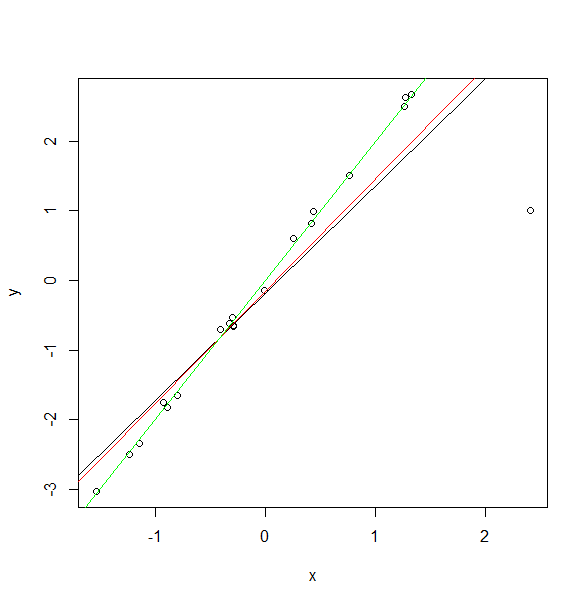
\includegraphics[width=8cm]{figures/trees-bagging-works-01}}
\end{example}

\begin{example}[Bagging on outliers, \#2]
The outlier (bad point) is a low-leverage point. Bootstrapping gives it more influence, slightly decreasing performance.

\centering{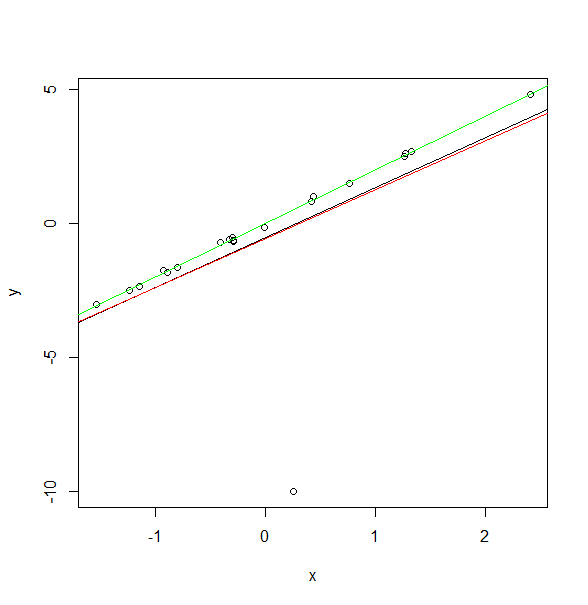
\includegraphics[width=8cm]{figures/trees-bagging-works-02}}
\end{example}

\begin{example}[Bagging on outliers, \#3]
The outlier (this time it's a good point) is a high-leverage point. Bootstrapping gives it less influence, slightly decreasing performance.

\centering{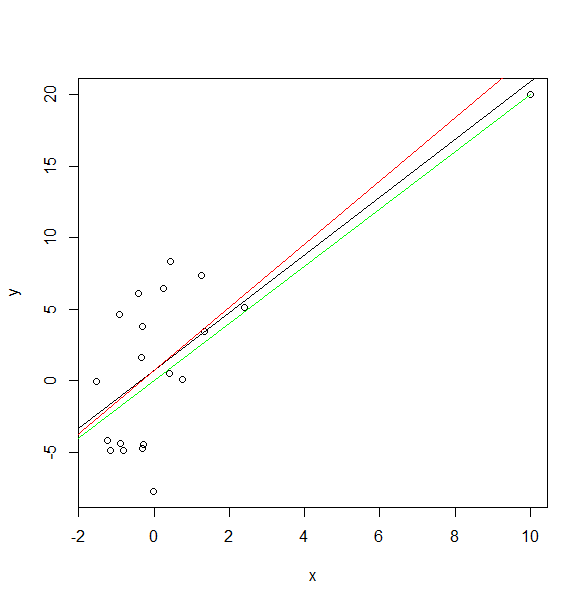
\includegraphics[width=8cm]{figures/trees-bagging-works-03}}
\end{example}

\section{Random Forests}

Random forests~\citep{Brieman2001} extend the idea of bagging but aim to develop even more de-correlated trees than those from bootstrap samples. The approach develops a possibly large collection of trees $\{T_b\}_1^B$, where each tree is inferred from a bootstrap sample of the training data set. To additionally diversify the trees, the features on which to split each internal node of the tree are selected from a random sample of $p$ variables. This is different from the normal growth of the trees which instead considers the entire set of predictors. Here, $p$ is a user-specified parameter. To make a prediction of a new data point $\vect{x}$, we either average the predictions of individual trees in a case of regression,
$$ \hat{f}_{\rm rf}^B(\vect{x})={1\over B}\sum_{b=1}^B T_b({\vect{x}}) $$
or choose a class using a majority vote in the case of classification.

Trees are ideal for the described averaging procedure. If they are grown sufficiently deep, they have a relatively low bias. As they are notoriously noisy, they can benefit from averaging. Since each tree in bagging is identically distributed, the expectation of an average of $B$ such trees is the same as the expectation of any of them. The bias of the bagged trees is the same as that of the individual trees. Hence, in random forests, it is recommended that the trees are not pruned but instead developed to the depth.

The benefits of trees can also be examined from the viewpoint of variance. Notice that the average of $B$ i.i.d. random variables, each with a variance of $\sigma^2$, has a variance
$${1\over B}\sigma^2.$$
If the variables are only identically distributed but not necessarily independent with a positive pairwise correlation of $\rho$, the variance of the average is
$$\rho\sigma^2+{1-\rho\over B}\sigma^2.$$
The aim of the random forest is to reduce the variance. We see that with a large number of the trees and hence large values of $B$ we decrease the value of the second term in the variance as expressed above. The first term, $\rho\sigma^2$, can then only be minimized by minimizing $\rho$. Hence, we prefer the trees that are different, and whose correlations in predictions is minimized. We, of course, prefer accurate trees, but those whose precision is focused on different parts of the parameter space. For this reason, besides bootstrap sampling, random forests engage extra randomization procedures, like arbitrarily choosing $p$ features when examining which feature to use at each split. In practice, $p$ can be relatively small and equal to $p=\sqrt{D}$ for classification and $p=D/3$ for regression.

Random forests do remarkably well in terms of accuracy, with very little or no tuning required~\citep{Fernandez-Delgado2014}. Just like trees, they require almost no data preprocessing, can treat both continuous and discrete features, and can easily handle missing values. The inference of trees is fast and can be applied to any reasonably sized data set. With these characteristics, random forests are a great baseline, that is, provide accuracies that need to be surpassed by more advanced approaches.

\subsection*{Out-of-Bag Estimates}

Bootstrap sampling, on the average, leaves $e^{-1}=0.368$ of data instances out of sample. An out-of-bag estimate is the mean prediction error on each training sample $\vect{x}_i$, using only the trees that did not have $\vect{x}_i$ in their bootstrap sample. With a fixed number of trees $B$ in the forest, this estimate would converge to the estimate we would obtain through, say, cross-validation. Alternatively, we can use the out-of-bag estimate to observe the convergence of estimated error and stop the growth of the trees when the error stabilizes. In practice, forests are usually grown to include up to a few hundreds of trees.

\subsection*{Estimate of Feature Importance}

One of the deficiencies of random forests is their overall complexity. If we agree that the trees are models that can be read and interpreted, we lose this ability with the forest simply because of the large collection of trees. With forests, interpretability is lost. To remedy the loss of interpretability, the author of the forests, \citet{Brieman2001}, proposes to provide estimates of the importance of features in the forests using out-of-bag estimates. The procedure randomly permutes the value of a selected feature and estimates the out-of-bag error. The decrease of accuracy caused by random permutation now provides an estimate of the feature's importance. Notice that estimates obtained in this way can be substantially different from univariate estimates of the correlation between a feature and a class variable, taking into account possible feature interactions discovered by the trees in the forest.


\printbibliography[heading=subbibliography]
\end{refsection}
